% !TeX root = 0-Introduction.tex

\documentclass[11pt,class=article,float=false,crop=false]{standalone}
\usepackage{0-Introduction_packages}

\begin{document}

\part*{Introduction}

Le Département des Matériaux pour le Nucléaire de la Direction des Énergies Nucléaires du CEA (DEN/DMN) étudie et analyse le comportement des matériaux utilisés dans les centrales nucléaires. Le département différencie l'étude des matériaux irradiés (SEMI) et la recherche en métallurgie appliquée (SRMA) en deux services incluant chacun plusieurs laboratoires d'étude et d'analyse. Le Laboratoire d'étude de Comportement Mécanique des Matériaux (LC2M), dans lequel j'effectue ma thèse, est chargé de la caractérisation mécanique des matériaux de l'industrie nucléaire.

Les études menées au LC2M ont pour but d'étudier le comportement dans matériaux utilisés au sein des installations nucléaires actuelles et futures. Des modèles de comportement sont développés pour mieux prédire les changements que traverseront les matériaux au cours de leur cycle de vie. Ces modèles prédisent notamment la réponse des matériaux aux conditions d'irradiation, de forte contrainte physique et de température que l'on peut observer dans ce type d'installations.

\subsection*{Matériaux étudiés}

Les matériaux étudiés sont les différents aciers qui composent les éléments des centrales, comme la cuve (Fig. \ref{fig:cuve}), et d'autre matériaux plus spécifiques comme les alliages de Zirconium utilisés pour les gaines de combustible (Fig. \ref{fig:gaine_zr}).

\begin{figure}[H]
	\centering
	\begin{subfigure}[b]{0.49\textwidth}
		\centering
		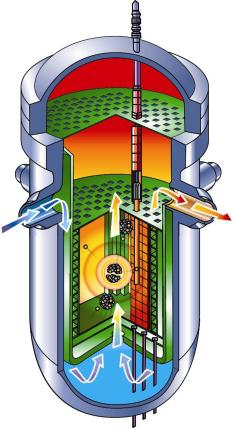
\includegraphics[height=0.3\textheight]{img/cuve}
		\caption{Cuve en acier d'un réacteur nucléaire.}
		\label{fig:cuve}
	\end{subfigure}
	\begin{subfigure}[b]{0.49\textwidth}
		\centering
		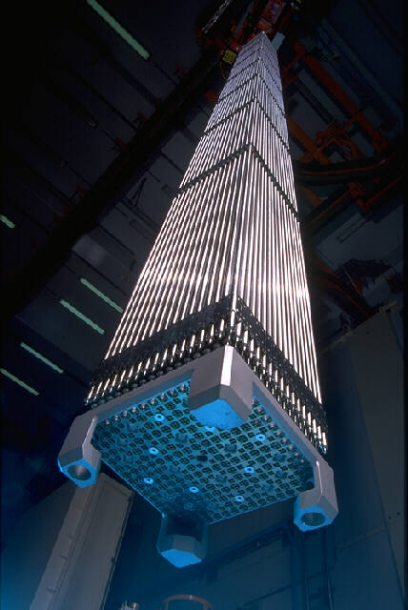
\includegraphics[height=0.3\textheight]{img/fuel_assembly}
		\caption{Assemblage de gaines de Zirconium.}
		\label{fig:gaine_zr}
	\end{subfigure}
	\caption{Matériaux étudiés au LC2M}
\end{figure}

La cuve d'un réacteur à eau pressurisée est l'élément principal du circuit primaire, et contient de l'eau dans laquelle baigne l'assemblage de combustible. Elle mesure une dizaine de mètres de haut pour quelques mètres de diamètre et est réalisée en acier faiblement allié  recouvert par une couche protectrice d'acier inoxydable. L'acier composant la structure principale de la cuve lui permet de résister aux fortes contraintes physiques (Pression, température, \dots) que doit supporter la cuve. L'acier pur lui confère de plus une résistance accrue aux dommages causés par l'irradiation. L'intérieur de la cuve, quand à lui, est recouvert d'une couche protectrice d'acier inoxydable permettant d'améliorer la résistance à la corrosion. Le processus de fabrication complexe et la robustesse dont doit faire preuve cet élément nécessite d'avoir une connaissance parfaite du comportement du matériau au cours du temps. Les études menées au CEA visent à garantir l'intégrité de la cuve tout au long de son cycle de vie.

L'assemblage de combustible est composé de nombreuses gaines en Zirconium contenant des pastilles de combustible. Les propriétés physique et la faible absorption des neutrons du Zirconium font de lui un candidat idéal pour contenir le combustible tout en permettant aux neutrons qui entretiennent la fission de circuler librement à travers l'assemblage. La proximité de ces éléments avec le combustible les rend particulièrement sensibles aux dommages dus à l'irradiation. Les études menées au CEA visent à comprendre et modéliser le comportement de ces éléments sous irradiation, notamment les mécanismes de fluage pouvant allonger les gaines de Zirconium de plusieurs centimètres au cours de leur cycle de vie.

%https://www.college-de-france.fr/media/jean-marie-tarascon/UPL18061_Expose_Nucleaire_YB.pdf
%http://areva.com/mediatheque/liblocal/docs/activites/reacteurs-services/equipements/pdf-plaq-creusot-vf.pdf
%http://www.irsn.fr/FR/connaissances/Installations_nucleaires/Les-centrales-nucleaires/cuves-reacteurs/Pages/2-caracteristiques-conception-fabrication-contrele-cuves.aspx#.WCBV37VuNhE
%https://tel.archives-ouvertes.fr/file/index/docid/419622/filename/SEKFALI.pdf
%https://tel.archives-ouvertes.fr/file/index/docid/688207/filename/19195_TREGO_2011_archivage.pdf
%http://www.irsn.fr/FR/Larecherche/publications-documentation/aktis-lettre-dossiers-thematiques/RST/RST-2005/Documents/F4RST05-3.pdf
%http://www.iaea.org/inis/collection/NCLCollectionStore/_Public/40/086/40086014.pdf
\subsection*{Études menées}
Des études expérimentales permettent de caractériser de manière empirique le comportement des matériaux, et la simulation informatique permet comprendre les phénomènes qui adviennent au cœur de la matière, notamment grâce à la modélisation multi-échelle.

\begin{figure}[H]
	\centering
	\begin{subfigure}[b]{0.33\textwidth}
		\centering
		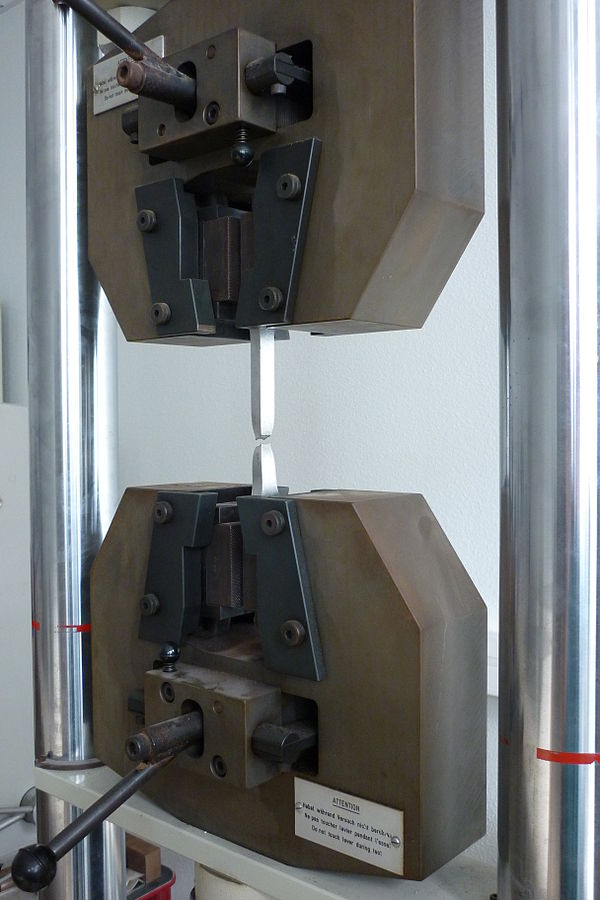
\includegraphics[height=7cm]{img/essai-traction.jpg}
		\caption{Machine de traction.}
		\label{fig:exp_lc2m:machine}
	\end{subfigure}	
	\begin{subfigure}[b]{0.66\textwidth}
		\centering
		\includestandalone[mode=tex,height=7cm]{img/stress-strain}
		\caption{Courbe Contrainte/Déformation.}
		\label{fig:exp_lc2m:courbe}
	\end{subfigure}
	\caption{Expérience et résultats d'un essai de traction.}
	\label{fig:exp_lc2m}
\end{figure}

\paragraph{Études expérimentales}
Les expérimentations menées au LC2M sont principalement des campagnes de caractérisation mécanique des matériaux. Elles consistent à observer la réponse des matériaux aux contraintes qui leurs sont appliquées. Parmi les expériences menées, nous pouvons citer des essais de traction, de fluage, d'éclatement, de fatigue, de résilience et de ténacité. A titre d'exemple, la figure \ref{fig:exp_lc2m} illustre un essai de traction. Dans cette expérience, l'échantillon est étiré par la machine de traction (\subref{fig:exp_lc2m:machine}). Les valeurs de l'allongement ainsi que la force appliquée sont enregistrées tout au long de l'expérience. Elles sont ensuite présentées sous forme d'une courbe contrainte/déformation (\subref{fig:exp_lc2m:courbe}). La déformation est le ratio d'allongement du matériau $\epsilon = \frac{\Delta l}{l}$ et la contrainte mesure la force appliquée sur l'échantillon par unité de surface $\sigma = \frac{F}{S}$.

Les autres laboratoires du service mettent aussi en œuvre des moyens d'expérimentation et d'observation, et travaillent aussi sur l'élaboration de nouveaux matériaux innovants. Le LA2M, par exemple possède un Microscope Électronique en Transmission (MET) qui permet d'observer la matière à l'échelle de l'atome. La Figure \ref{fig:MET} montre une image produite par un MET dans laquelle on peut observer un réseau de dislocations et des boucles d'irradiation. Ces images ont été produites par J. \textsc{Drouet} dans le cadre de sa thèse \citeintro{drouet2016comparaison-intro}.

\begin{figure}[H]
  \centering
  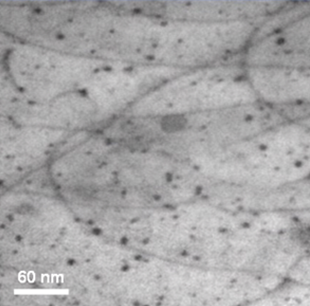
\includegraphics[height=0.3\textheight]{img/dislocations-MET}
  \caption[Dislocations au MET]{Images de dislocation MET in-situ \citeintro{drouet2016comparaison-intro}}
  \label{fig:MET}
\end{figure}

\paragraph{Modélisation et simulation}
Les études expérimentales sont complétées par de la modélisation et la simulation. L'utilisation de modèles et d'outils informatiques permet de réduire le coût et le temps nécessaire pour mener à bien les campagnes de caractérisation des matériaux. En particulier, la simulation complète avantageusement les études sur les matériaux irradiés très coûteux à produire. Ce type d'études nécessite la préparation d'échantillons au sein de réacteurs expérimentaux dont l'exploitation est très coûteuse. La manipulation de tels échantillons nécessite du matériel de pointe. 

Par des techniques de visualisation, la simulation permet d'observer certains phénomènes difficilement observables en conditions réelles. %Par exemple la figure \ref{fig:numodis-intro} présente le résultat d'une simulation de Dynamique des Dislocations par le logiciel NuMoDis.

% \begin{figure}[H]
%   \centering
%   \includegraphics[height=0.3\textheight]{img/numodis-intro}
%   \caption{Visualisation d'une simulation de Dynamique des Dislocations.}
%   \label{fig:numodis-intro}
% \end{figure}

L'enjeu de la simulation des phénomènes physiques est de proposer une modélisation fidèle du comportement des matériaux à moindre coût. La simulation multi-échelle modélise le comportement des matériaux en décrivant les interactions les plus élémentaires pour ensuite monter en échelle afin de modéliser des systèmes de plus en plus complexes. Les méthodes utilisées vont de la Dynamique Moléculaire aux simulations Éléments Finis ou FFT en passant par la Dynamique des Dislocations.

La Dynamique des Dislocations étudiée au cours de cette thèse se place à une échelle intermédiaire. Elle modélise le comportement des défauts présents dans la structure des matériaux cristallins. Il s'agit d'un maillon essentiel de la simulation multi-échelle et pose de nombreux défis dans le domaine de la mécanique des matériaux, mais aussi dans celui de l'informatique. L'objectif de cette thèse et de répondre à certains des défis informatiques que pose la simulation massive de Dynamique des Dislocations sur des calculateurs massivement parallèles.

%http://www-cast3m.cea.fr/
\bibliographystyleintro{plain}
\bibliographyintro{0-Introduction_biblio}

\end{document}